\documentclass[12pt]{article}
\usepackage{amsmath}
\usepackage{graphicx}
\usepackage{caption}
\usepackage{subcaption}
\usepackage{booktabs}
\usepackage{float}
\usepackage[utf8]{inputenc}
\usepackage{geometry}[a4paper, margin=1in]
\usepackage{multirow}
\usepackage{setspace}
\usepackage{parskip}
\usepackage{svg}
\usepackage[bottom]{footmisc}
\usepackage{tikz}
\usepackage[section]{placeins}
\usepackage{pgfplots}
\usepackage[caption=false]{subfig}
\usepackage{tocloft}
\usepackage{hyperref}

\usepackage{lipsum} % For dummy text



% This style is used to create block diagrams, you'll find it useful since many of your figures would be of that form, I'll try add more styles in the future :)
\usetikzlibrary{trees,positioning,fit,calc}
\tikzset{block/.style = {draw, fill=blue!20, rectangle,
                         minimum height=3em, minimum width=4em},
        input/.style = {coordinate},
        output/.style = {coordinate}
}

\usepackage[section]{minted}
\usepackage{xcolor}
\usemintedstyle{borland}

\counterwithin{figure}{section}
\counterwithin{table}{section}
\counterwithin{listing}{section}

\renewcommand{\arraystretch}{1.5}

\usepackage[hidelinks]{hyperref}
\hypersetup{
    linktoc=all
}

\renewcommand\listingscaption{Listing}

\usepackage{tocbasic}
\setuptoc{lol}{levelup}

\setlength{\parindent}{0em}
\setlength{\parskip}{0em}

\newlistof{listoftables}{lot}{List of Tables}

% Define a new command to add entries to the table of tables
\newcommand{\addtotables}[1]{%
  \addcontentsline{lot}{table}{#1}}


%----------EDIT COVER INFO HERE -----------------%

\def \LOGOPATH {assets/birzeit-logo.svg}
\def \FACULTY {Faculty of Engineering and Technology}
\def \DEPARTEMENT {Department of Electrical and Computer Engineering}
\def \COURSENUM {ENCS5343}
\def \COURSENAME {Computer Vision }
\def \ASSIGNMENTTITLE {Project }
\def \ASSIGNMENTDESCRIPTION {Arabic Handwriting Identification Using Deep Learning }
\def \STUDENTNAME {\\Ahmad Hamad 1212621 \\  Mohammed Abed Alkareem }
\def \STUDENTID {1210708}
\def \INSTRUCTOR {Dr.Aziz Qaroush}
% \def \ASSISTANT {Ahmad Abbas}

%------------------------------------------------%

\begin{document}

\pagenumbering{Roman}

\begin{titlepage}
    \vfill
    \begin{center}
        \includesvg[width=0.7\textwidth]{\LOGOPATH} \\
        \hfill \\
        \Large{\FACULTY} \\
        \Large{\DEPARTEMENT} \\
        \Large{\COURSENUM\textemdash\COURSENAME} \\
        \vfill
        \textbf{\LARGE{\ASSIGNMENTTITLE\textemdash\ASSIGNMENTDESCRIPTION}} \\
        \vspace{20pt}
        \Large{\textbf{Prepared by:} \STUDENTNAME\textemdash\STUDENTID}
    \end{center}
    \vfill
    \begin{flushleft}
        \Large{\textbf{Instructor:} \INSTRUCTOR} \\
        % \Large{\textbf{Assistant:} \ASSISTANT} \\
        \Large{\textbf{Date:} \today}
    \end{flushleft}
\end{titlepage}

%--------------ABSTRACT ------------------------%

\section*{Abstract}
\label{sec:abstract}
\addcontentsline{toc}{section}{\protect\numberline{}\nameref{sec:abstract}}

The aim of this project is to experiment optimizing different convolutional neural network (CNN) architectures for identifying Arabic handwritten Writers, it involves designing custom network, data augmentation, and transfer learning. Initially, various CNN models are designed and trained with hyperparameter tuning, evaluating parameters such as convolutional filters, pooling strategies, and training configurations. The simplest and most effective network is selected based on accuracy and loss trends.
The selected model is further enhanced using data augmentation techniques like flipping, rotation, scaling and illuminating to improve generalization. The Project continues by using standard published CNN architecture for training on the augmented dataset to compare performance. Finally, A pre-trained CNN is fine-tuned using transfer learning to leverage prior knowledge from similar tasks, achieving improved accuracy and efficiency.
This progressive methodology highlights the benefits of architectural optimization, data augmentation, and transfer learning in developing effective CNN models.

\clearpage

%-----------------------------------------------%

\tableofcontents
\clearpage

\listoffigures

\clearpage

\listoftables
\clearpage



\setlength{\parskip}{\baselineskip}%

\pagenumbering{arabic}

\section{Introduction}
% \subsection*{Motivation}
% Diabetes is a chronic disease that poses significant health risks, affecting millions of people globally. Early and accurate classification of diabetes types is essential for personalized treatment, effective management, and reducing long-term complications. Despite advances in medical diagnostics, the complexity and variability of diabetes markers necessitate leveraging machine learning techniques to improve classification accuracy. This study is motivated by the need to harness the power of data-driven approaches to provide reliable tools for healthcare professionals, potentially leading to better patient outcomes and efficient healthcare delivery.

\subsection{Dataset}
The \textbf{AHAWP (Arabic Handwritten Automatic Word Processing) Dataset} is a benchmark for handwritten Arabic text recognition. It contains 8,144 word-level images of 10 unique words, each handwritten by 82 individuals with 10 samples per word. Writers are anonymized with unique IDs, ensuring privacy. This diverse dataset is ideal for evaluating local feature extraction algorithms like SIFT and ORB.

\subsection{Convolutional Neural Networks (CNNs)}
Convolutional Neural Networks (CNNs) are deep learning models ideal for image processing tasks. They automatically learn spatial hierarchies of features through convolutional layers, which detect local patterns like edges and shapes. Key attributes include:
\begin{itemize}
    \item \textbf{Convolutional Layers:} Extract features like edges and shapes by applying filters across the input, enabling hierarchical feature learning.
    \item \textbf{Pooling Layers:} Reduce spatial dimensions while retaining key information, improving efficiency. Common types include max and average pooling.
    \item \textbf{Activation Functions:} Introduce non-linearity for learning complex patterns. Examples include ReLU, sigmoid, and tanh.
    \item \textbf{Fully Connected Layers:} Map extracted features to output classes or predictions, learning global relationships.
    \item \textbf{Local Connectivity:} Focus on small input regions to capture spatial hierarchies and reduce parameters.
    \item \textbf{Parameter Sharing:} Use the same filters across the input, improving generalization and reducing model size.
\end{itemize}

\clearpage

\subsection{Augmentaion \& its Importance}
Data augmentation is a technique used to artificially expand the size and diversity of a dataset by applying transformations such as rotation, flipping, cropping, scaling, and color adjustments to the existing data. This is particularly valuable in scenarios where datasets are small, as it helps to improve the model's generalization and robustness by exposing it to varied versions of the data. Deep learning models are inherently data-hungry and tend to perform poorly on limited data due to their high capacity and propensity to overfit. Augmentation mitigates this issue by creating a richer training set, effectively improving model performance without the need for additional data collection.

\subsection{Popular Architectures}
\subsubsection{ResNet-18  }
ResNet-18 is a deep convolutional neural network known for introducing residual connections, which help mitigate the vanishing gradient problem in deep networks. With 18 layers, it is relatively lightweight compared to deeper ResNet variants, making it suitable for tasks requiring a balance between performance and computational efficiency. ResNet-18 employs residual blocks with shortcut connections that allow gradients to flow more easily during backpropagation, ensuring stable training and improved accuracy on image classification and other vision tasks.

\subsubsection{ResNet-50}
ResNet-50 is a deeper and more powerful variant of the ResNet family, with 50 layers organized into residual blocks. It is particularly effective for complex computer vision tasks, such as object detection and image segmentation, due to its increased capacity for feature learning. ResNet-50 uses bottleneck residual blocks, which reduce computational cost by downsampling the input dimensions before applying convolutions and then restoring them. This architecture strikes a good balance between depth and efficiency, making it widely adopted for both academic research and industry applications.

\subsubsection{MobileNetV3-Large}
MobileNetV3-Large is an efficient deep learning model designed for mobile and edge devices, balancing high accuracy with low computational requirements. It combines techniques like depthwise separable convolutions, squeeze-and-excitation blocks, and the swish activation function to enhance performance. The "Large" variant provides higher accuracy compared to the "Small" variant, making it suitable for more demanding tasks while still being optimized for resource-constrained environments. MobileNetV3-Large is commonly used in applications such as image recognition and object detection on devices with limited hardware capabilities.



\subsection{Pre-trained Model and Fine-tuning}
To enhance character recognition on the AHAWP dataset, we fine-tuned a pre-trained resnet and mobile net models which are pre-trained on Image net dataset by loading these models and initialize them with their pre-trained weights . The original models were trained on 1000 classes, but we adapted it to our 82-class dataset by retraining. This fine-tuning aligned the model's predictions with our dataset's class structure, improving its performance in recognizing characters.






\section{Experimental Setup and results }

The study starts by preparing the data, the dataset comprises 82 classes, with each class contributing in the text writer recognition and classification.


\section*{Dataset Preprocessing}
The preprocessing for the AHAWP (Arabic Handwritten Automatic Word Processing) Dataset involves several steps to ensure uniformity and compatibility with the deep learning model. First, each image is resized to a standard dimension of 224x224 pixels, addressing the lack of a consistent image size in the dataset. The images are then converted to grayscale, reducing them to a single channel to focus on intensity values without color information. Next, pixel values are normalized to have a mean of 0.5 and a standard deviation of 0.5, ensuring that the data is centered and scaled, which helps accelerate convergence during training. The dataset is organized using PyTorch's `ImageFolder` class, and then split into training (64\%), validation (16\%), and testing (20\%) subsets to evaluate model performance. Data loaders are defined for each subset, with a batch size of 256, enabling efficient data handling during training and evaluation. Finally, a sample of images from the dataset was visually inspected to verify the pre-processing steps and observe the quality and characteristics of the handwritten data.

\section*{Training process}
The training process involves iterating through the training dataset for a specified number of epochs (default of 100), where each batch undergoes a forward pass through the model, and the loss is calculated using the specified criterion. The optimizer then adjusts the model's parameters based on the loss. During each epoch, the training loss and accuracy are calculated, providing insights into the model's learning progress. The model is also evaluated on the validation dataset after each epoch to monitor its generalization performance. The evaluation involves computing the validation loss and accuracy by passing the validation data through the model without gradient calculation. Early stopping is implemented with default parameters (patience=6, min delta=0.001), which halts training if the validation loss does not improve for 6 consecutive epochs. This strategy ensures the model achieves the best possible performance without excessive training.

\section*{Evaluation Methodology}
The evaluation methodology in this context involves monitoring the model's performance during training and validation through key metrics—loss and accuracy. During each epoch, the model's training and validation loss are computed. The training loss reflects how well the model is fitting the training data, while the validation loss indicates how well the model generalizes to unseen data. Similarly, the training and validation accuracy are tracked to gauge the percentage of correct predictions during each phase. Early stopping is applied to prevent overfitting, halting the training if the validation loss does not improve for a specified number of consecutive epochs.

To visualize the performance across epochs, two plotting functions are used: \texttt{plot\_loss\_per\_epoch} and \texttt{plot\_accuracy\_per\_epoch}. These functions display how the loss and accuracy evolve over time for both the training and validation sets. This provides a clear view of whether the model is learning effectively and if overfitting or underfitting occurs. The plots help in understanding the balance between training performance and generalization, guiding the user in evaluating the model’s effectiveness throughout the training process.


\section*{Task 1 Customized CNN training \& Evaluation}
Multiple customized CNN architectures, each featuring a different number of convolutional layers, activation functions, pooling layers, kernel sizes, strides, and additional parameters, are explored to identify the optimal model. To further fine-tune performance, advanced optimizers such as Adam and AdamW are employed. Below are the detailed models and their respective architectures.

\subsubsection*{NetCNN\_0}

\begin{itemize}
    \item \textbf{Input:} \(1 \times 224 \times 224\) (grayscale image).
    \item \textbf{Convolutional Layers:} 3 layers with increasing channels (\(1 \to 10 \to 40 \to 80\)), kernel size \(3 \times 3\), padding \(1\), and ReLU activation.
    \item \textbf{Pooling Layers:} Max-pooling (\(2 \times 2\)) after each convolution, reducing dimensions: \(224 \to 112 \to 56 \to 28\).
    \item \textbf{Fully Connected Layers:} 
    \begin{itemize}
        \item Flattens (\(28 \times 28 \times 80 = 62,720\)).
        \item 4 dense layers with ReLU activation (\(64 \to 128 \to 256 \to \text{num\_classes}\)).
    \end{itemize}
    \item \textbf{Evaluation}
\end{itemize}

% \usepackage{subcaption}

\begin{figure}[ht]
    \centering
    \begin{subfigure}{0.45\linewidth}
        \centering
        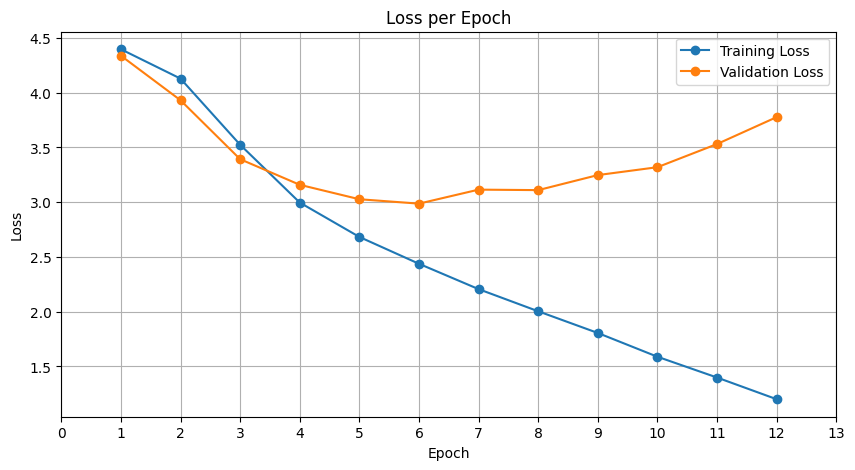
\includegraphics[width=\linewidth]{net0_loss.png}
        \caption{Net 0 CNN val vs training loss}
        \label{fig:net0_loss}
    \end{subfigure}
    \hfill
    \begin{subfigure}{0.45\linewidth}
        \centering
        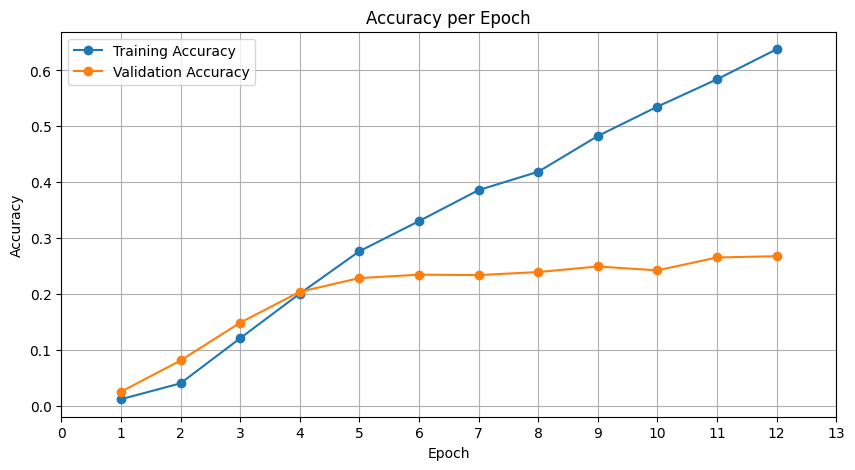
\includegraphics[width=\linewidth]{net0_CNN_Acc.png}
        \caption{Net 0 CNN training vs val acc}
        \label{fig:net0_CNN_Acc}
    \end{subfigure}
    \caption{Comparison of Net 0 CNN performance}
    \label{fig:net0_CNN_performance}
\end{figure}

The model achieved a training accuracy of \textbf{80.3\%} but a significantly lower validation accuracy of \textbf{30.3\%}, with early stopping applied at epoch \textbf{12}. This large gap between training and validation accuracy indicates \textbf{overfitting} as it fails to generalize to unseen data. Potential reasons for this performance include the relatively small dataset size and the high capacity of the model, which may require regularization techniques or data augmentation to improve generalization.



\subsubsection*{NetCNN\_1}

\begin{itemize}
    \item \textbf{Input:} \(1 \times 224 \times 224\) (grayscale image).
    \item \textbf{Convolutional Layers:} 2 layers with channels (\(1 \to 16 \to 32\)), kernel size \(3 \times 3\), padding \(1\), ReLU activation.
    \item \textbf{Pooling Layers:} Max-pooling (\(2 \times 2\)) after each convolution, reducing dimensions: \(224 \to 112 \to 56\).
    \item \textbf{Fully Connected Layers:} 
    \begin{itemize}
        \item Flattens (\(32 \times 56 \times 56 = 100,352\)).
        \item 2 dense layers with ReLU activation (\(256 \to \text{num\_classes}\)).
    \end{itemize}
\end{itemize}

% \usepackage{subcaption}

\begin{figure}[ht]
    \centering
    \begin{subfigure}{0.45\linewidth}
        \centering
        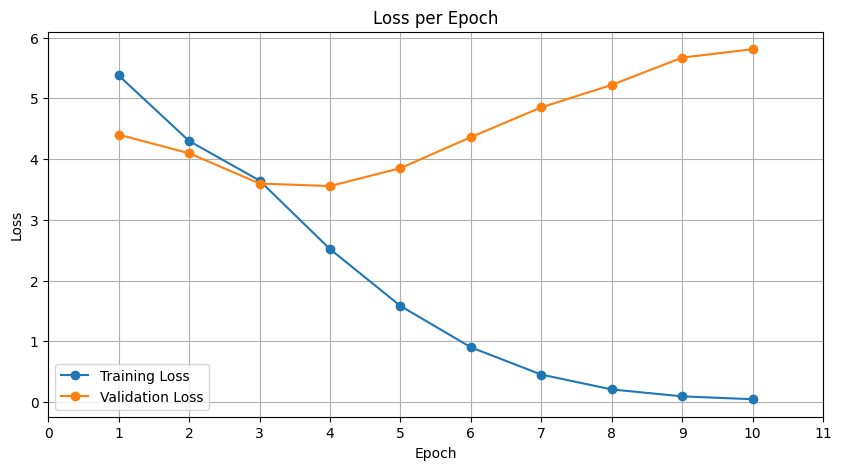
\includegraphics[width=\linewidth]{net_1_loss.png}
        \caption{Net 1 CNN val vs training loss}
        \label{fig:net0_loss}
    \end{subfigure}
    \hfill
    \begin{subfigure}{0.45\linewidth}
        \centering
        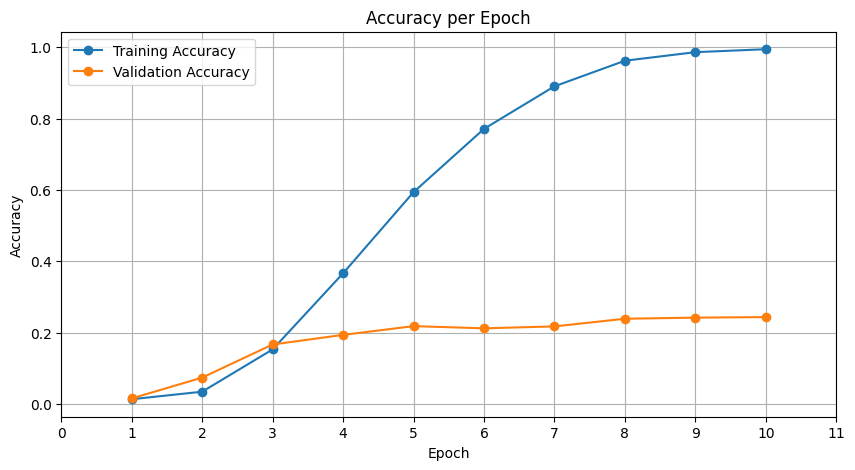
\includegraphics[width=\linewidth]{net1_acc.png}
        \caption{Net 1 CNN training vs val acc}
        \label{fig:net0_acc}
    \end{subfigure}
    \caption{Net 1 CNN performance metrics}
    \label{fig:net0_performance}
\end{figure}

The model achieved a training accuracy of \textbf{99.4\%} at epoch 10, but the validation accuracy was significantly lower at \textbf{24.3\%}. Early stopping was applied at epoch 12 due to the validation loss increasing, indicating \textbf{overfitting}. This large gap between training and validation accuracy suggests that the model fails to generalize to unseen data. Potential reasons for this performance include the relatively small dataset size and the high capacity of the model, which may require regularization techniques or data augmentation to improve generalization. NetCNN\_1 introduces shallower netwrok to improve training stability and reduce overfitting.


% \section*{Key Differences}
% \begin{itemize}
%     \item \textbf{NetCNN\_0:} More complex with 3 convolutional layers and deeper fully connected layers.
%     \item \textbf{NetCNN\_1:} Simpler with 2 convolutional layers and a smaller fully connected network.
% \end{itemize}


% \begin{document}

\section*{NetCNN\_2}
This model is a Convolutional Neural Network (CNN) with the following characteristics:
\begin{itemize}
    \item \textbf{Three convolutional layers}, each followed by batch normalization, ReLU activation, and average pooling.
    \item \textbf{Average Pooling} with a kernel size of 2 and a stride of 2.
    \item \textbf{Padding=0} in all convolution layers.
    \item \textbf{Dropout layer} with a probability of 0.4 to avoid overfitting.
    \item The \textbf{fully connected (FC) layers} follow the convolutional layers, where the output from the convolution layers is flattened and passed through two fully connected layers with 512 and 82 output features respectively.
    \item Input size: \textbf{1 x 224 x 224}.
\end{itemize}

The architecture can be summarized as follows:

\[
\text{Input (1 x 224 x 224)} \xrightarrow{\text{Conv2d}} 16 \times 222 \times 222 \xrightarrow{\text{BatchNorm, ReLU}} \xrightarrow{\text{AvgPool}} 16 \times 111 \times 111
\]

\[
\text{Conv2d} \rightarrow 32 \times 109 \times 109 \xrightarrow{\text{BatchNorm, ReLU}} \xrightarrow{\text{AvgPool}} 32 \times 54 \times 54
\]

\[
\text{Conv2d} \rightarrow 64 \times 52 \times 52 \xrightarrow{\text{BatchNorm, ReLU}} \xrightarrow{\text{AvgPool}} 64 \times 26 \times 26
\]

\[
\text{Fully Connected Layer} \rightarrow \text{512 units} \rightarrow \text{82 units (num\_classes)}
\]

\textbf{Evaluation}

\begin{figure}[ht]
    \centering
    \begin{subfigure}{0.45\linewidth}
        \centering
        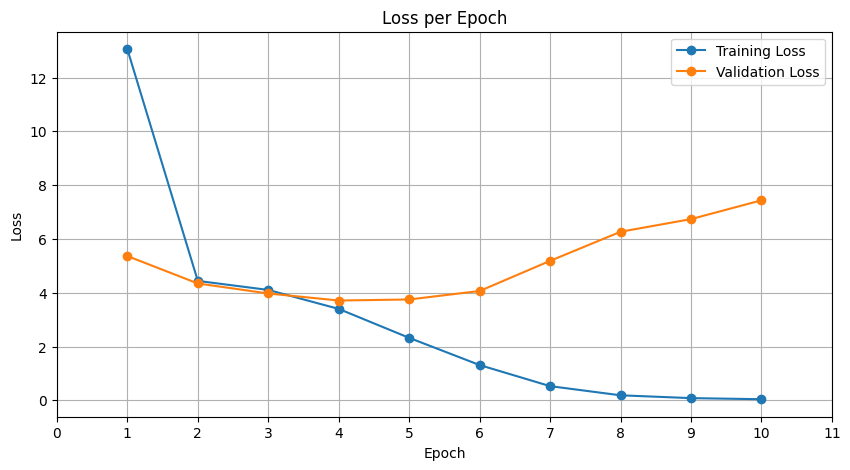
\includegraphics[width=\linewidth]{net2_loss.png}
        \caption{Net 2 CNN val vs training loss}
        \label{fig:net2_loss}
    \end{subfigure}
    \hfill
    \begin{subfigure}{0.45\linewidth}
        \centering
        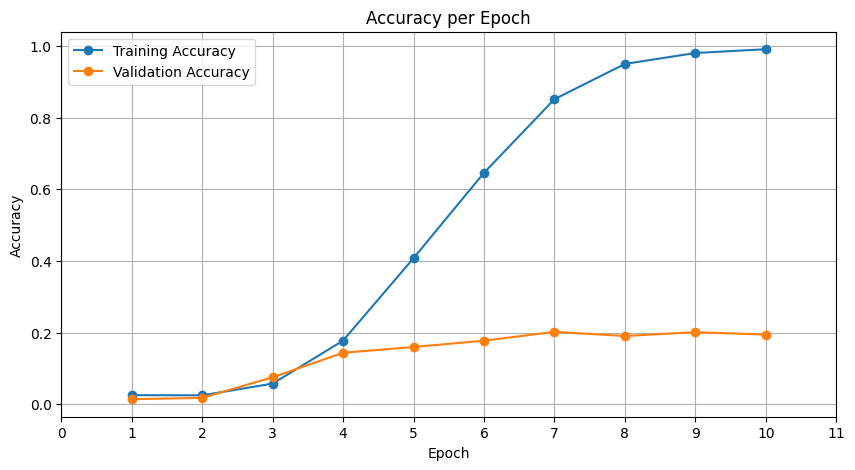
\includegraphics[width=\linewidth]{net2_acc.png}
        \caption{Net 2 CNN training vs val acc}
        \label{fig:net2_acc}
    \end{subfigure}
    \caption{Comparison of Net 2 performance}
    \label{fig:net2_performance}
\end{figure}

The model achieved a training accuracy of \textbf{99.1\%} at epoch 10, but the validation accuracy was significantly lower at \textbf{20.1\%}. Early stopping was applied at epoch 12 due to the validation loss increasing, indicating \textbf{overfitting}. This large gap between training and validation accuracy suggests that the model fails to generalize to unseen data. Potential reasons for this performance include the relatively small dataset size and the high capacity of the model, which may require regularization techniques or data augmentation to improve generalization. Compared to its predecessors, NetCNN\_2 introduces batch normalization and dropout layers to improve training stability and reduce overfitting.

\section*{NetCNN\_3}
This model follows a similar structure to NetCNN\_2, but with the addition of \textbf{Global Average Pooling (GAP)} to replace the fully connected layers. The key characteristics are:
\begin{itemize}
    \item \textbf{Three convolutional layers} with batch normalization, ReLU activation, and average pooling.
    \item \textbf{Global Average Pooling (GAP)} replaces the fully connected layers.
    \item \textbf{Dropout layer} with a probability of 0.4.
    \item The final output is passed through a single \textbf{linear layer} with output size equal to the number of classes (82).
    \item Input size: \textbf{1 x 224 x 224}.
\end{itemize}

The architecture can be summarized as follows:

\[
\text{Input (1 x 224 x 224)} \xrightarrow{\text{Conv2d}} 16 \times 222 \times 222 \xrightarrow{\text{BatchNorm, ReLU}} \xrightarrow{\text{AvgPool}} 16 \times 111 \times 111
\]

\[
\text{Conv2d} \rightarrow 32 \times 109 \times 109 \xrightarrow{\text{BatchNorm, ReLU}} \xrightarrow{\text{AvgPool}} 32 \times 54 \times 54
\]

\[
\text{Conv2d} \rightarrow 64 \times 52 \times 52 \xrightarrow{\text{BatchNorm, ReLU}} \xrightarrow{\text{AvgPool}} 64 \times 26 \times 26
\]

\[
\text{Global Average Pooling (GAP)} \rightarrow 64 \times 1 \times 1
\]

\[
\text{Fully Connected Layer} \rightarrow \text{82 units (num\_classes)}
\]


\textbf{Evaluation}
\begin{figure}[ht]
    \centering
    \begin{subfigure}{0.45\linewidth}
        \centering
        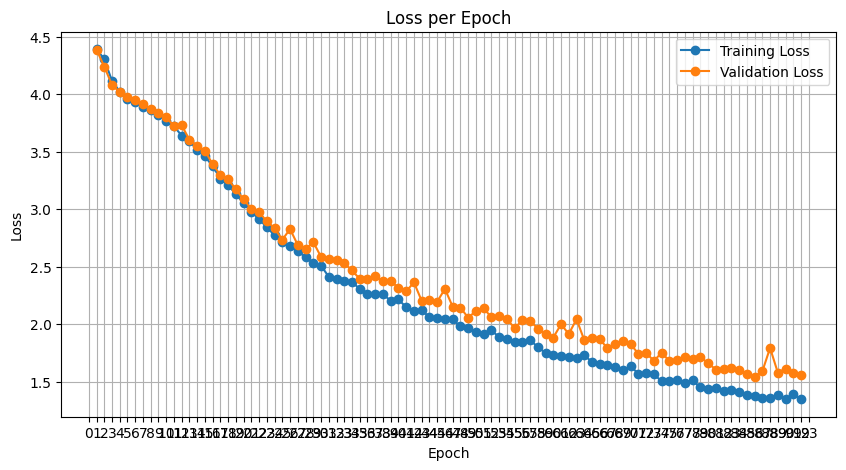
\includegraphics[width=\linewidth]{net3_loss.png}
        \caption{Net 3 CNN val vs training loss}
        \label{fig:net3_loss}
    \end{subfigure}
    \hfill
    \begin{subfigure}{0.45\linewidth}
        \centering
        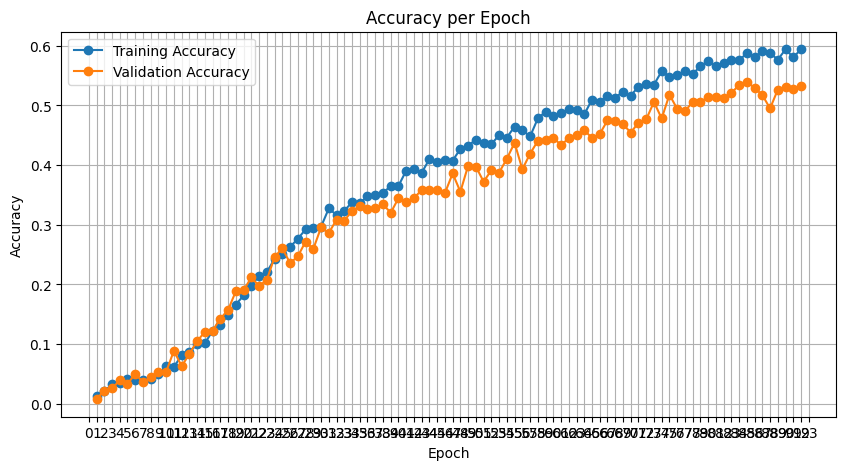
\includegraphics[width=\linewidth]{net3_acc.png}
        \caption{Net 3 CNN training vs val acc}
        \label{fig:net3_acc}
    \end{subfigure}
    \caption{Net 3 CNN performance metrics}
    \label{fig:net3_performance}
\end{figure}

The model achieved a training accuracy of \textbf{59.4\%} at epoch 92, but the validation accuracy was slightly lower at \textbf{54\%}. Potential reasons for this performance include the relatively small dataset size and the high capacity of the model, which may require regularization techniques or data augmentation to improve generalization. Compared to its predecessor, NetCNN\_2, which achieved a training accuracy of \textbf{99.1\%} and a validation accuracy of \textbf{20.1\%}, NetCNN\_3 shows a more balanced performance with a smaller gap between training and validation accuracy. NetCNN\_3 introduces \textbf{Global Average Pooling (GAP)} to replace the fully connected layers, aiming to reduce the number of parameters and potentially improve generalization.

\section*{NetCNN\_4}
This model utilizes \textbf{stride-2 convolutional layers} to downsample the input. It incorporates \textbf{Batch Normalization} and \textbf{Global Average Pooling}. The key characteristics are:
\begin{itemize}
    \item \textbf{Three convolutional layers} with stride=2, followed by batch normalization and ReLU activation.
    \item \textbf{Global Average Pooling} is applied to reduce the spatial dimensions to 1 x 1.
    \item The output of the \textbf{GAP layer} is passed through a \textbf{fully connected layer} to produce the final output.
    \item Input size: \textbf{1 x 224 x 224}.
\end{itemize}

The architecture can be summarized as follows:

\[
\text{Input (1 x 224 x 224)} \xrightarrow{\text{Conv2d}} 32 \times 112 \times 112 \xrightarrow{\text{BatchNorm, ReLU}} 
\]

\[
\text{Conv2d} \rightarrow 64 \times 56 \times 56 \xrightarrow{\text{BatchNorm, ReLU}} 
\]

\[
\text{Conv2d} \rightarrow 128 \times 28 \times 28 \xrightarrow{\text{BatchNorm, ReLU}} 
\]

\[
\text{Global Average Pooling (GAP)} \rightarrow 128 \times 1 \times 1
\]

\[
\text{Fully Connected Layer} \rightarrow \text{82 units (num\_classes)}
\]

\textbf{Evaluation}

\begin{figure}[ht]
    \centering
    \begin{subfigure}{0.45\linewidth}
        \centering
        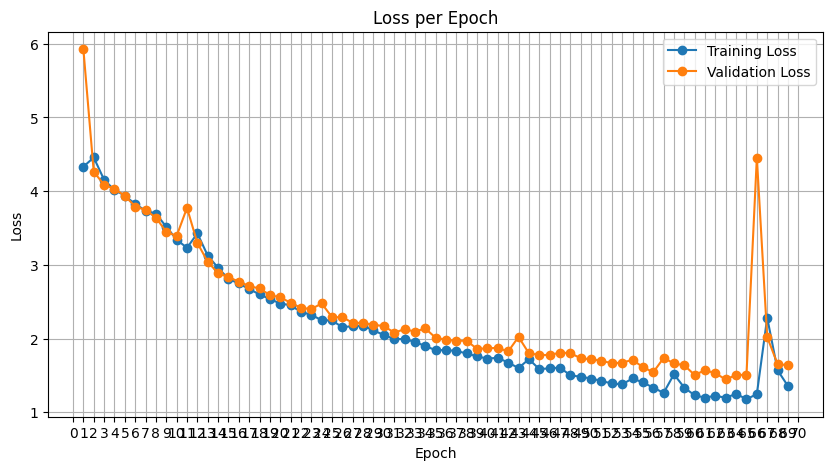
\includegraphics[width=\linewidth]{net4_loss.png}
        \caption{Net 4 CNN val vs training loss}
        \label{fig:net4_loss}
    \end{subfigure}
    \hfill
    \begin{subfigure}{0.45\linewidth}
        \centering
        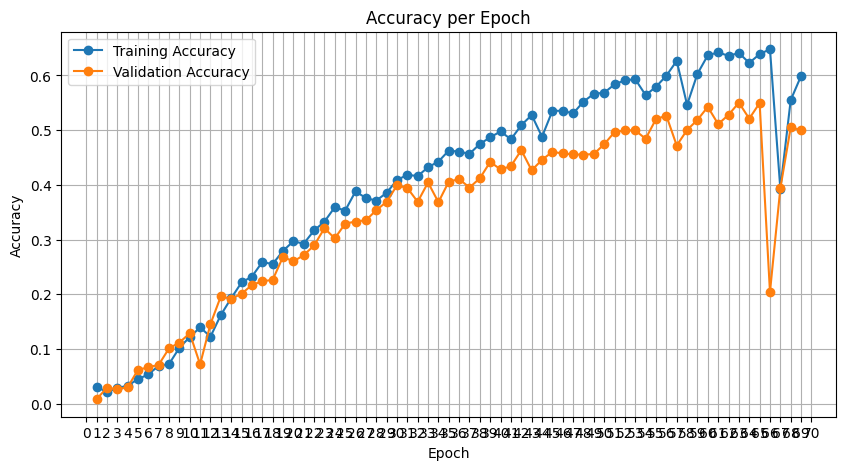
\includegraphics[width=\linewidth]{net4_acc.png}
        \caption{Net 4 CNN training vs val acc }
        \label{fig:net4_acc}
    \end{subfigure}
    \caption{Comparison of Net 4 performance}
    \label{fig:net4_performance}
\end{figure}

The model achieved a training accuracy of \textbf{59.9\%} at epoch 69, but the validation accuracy was slightly lower at \textbf{55\%}. Potential reasons for this performance include the relatively small dataset size and the high capacity of the model, which may require regularization techniques or data augmentation to improve generalization. Compared to its predecessor, NetCNN\_3, which achieved a training accuracy of \textbf{59.4\%} and a validation accuracy of \textbf{54\%}, NetCNN\_4 shows a slight improvement in both training and validation accuracy. NetCNN\_4 introduces \textbf{stride-2 convolutional layers} to downsample the input and \textbf{Global Average Pooling (GAP)} to reduce the spatial dimensions to 1 x 1, aiming to improve the model's efficiency and generalization.

\section*{NetCNN\_5}
This model uses \textbf{four convolutional layers} with varying pooling operations (MaxPool and AvgPool) and a kernel size of 3. The key characteristics are:
\begin{itemize}
    \item \textbf{Four convolutional layers} with alternating \textbf{MaxPool} and \textbf{AvgPool} operations.
    \item \textbf{Padding=1} in all convolution layers.
    \item \textbf{Batch normalization} and \textbf{ReLU activation}.
    \item \textbf{Fully connected layers} follow the convolutional layers, where the output is flattened and passed through two fully connected layers.
    \item Input size: \textbf{1 x 224 x 224}.
\end{itemize}

The architecture can be summarized as follows:

\[
\text{Input (1 x 224 x 224)} \xrightarrow{\text{Conv2d}} 16 \times 224 \times 224 \xrightarrow{\text{BatchNorm, ReLU}} \xrightarrow{\text{MaxPool}} 16 \times 112 \times 112
\]

\[
\text{Conv2d} \rightarrow 32 \times 112 \times 112 \xrightarrow{\text{BatchNorm, ReLU}} \xrightarrow{\text{AvgPool}} 32 \times 112 \times 112
\]

\[
\text{Conv2d} \rightarrow 64 \times 112 \times 112 \xrightarrow{\text{BatchNorm, ReLU}} \xrightarrow{\text{MaxPool}} 64 \times 56 \times 56
\]

\[
\text{Conv2d} \rightarrow 128 \times 56 \times 56 \xrightarrow{\text{BatchNorm, ReLU}} \xrightarrow{\text{AvgPool}} 128 \times 56 \times 56
\]

\[
\text{Fully Connected Layer} \rightarrow 512 \rightarrow 82 \text{ units (num\_classes)}
\]

\textbf{Evaluation}

\begin{figure}[ht]
    \centering
    \begin{subfigure}{0.45\linewidth}
        \centering
        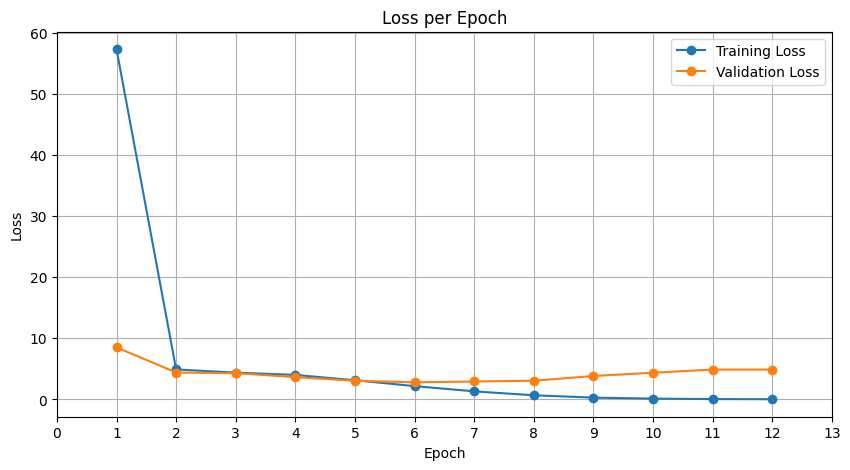
\includegraphics[width=\linewidth]{net5_loss.png}
        \caption{Net 5 CNN val vs training loss}
        \label{fig:net5_loss}
    \end{subfigure}
    \hfill
    \begin{subfigure}{0.45\linewidth}
        \centering
        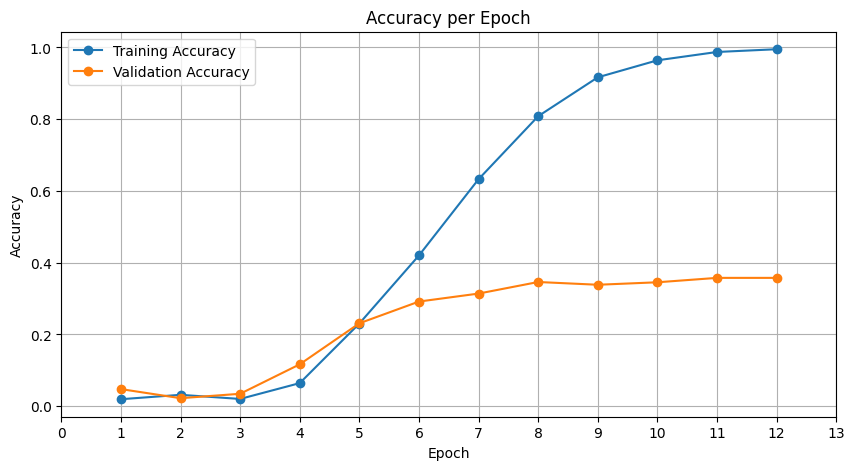
\includegraphics[width=\linewidth]{net5_acc.png}
        \caption{Net 5 CNN training vs val acc}
        \label{fig:net5_acc}
    \end{subfigure}
    \caption{Comparison of Net5 performance}
    \label{fig:net5_performance}
\end{figure}

The model achieved a training accuracy of \textbf{99.5\%} at epoch 12, but the validation accuracy was significantly lower at \textbf{35.8\%}. This large gap between training and validation accuracy indicates \textbf{overfitting}, suggesting that the model fails to generalize to unseen data. Potential reasons for this performance include the relatively small dataset size and the high capacity of the model, which may require regularization techniques or data augmentation to improve generalization. Compared to its predecessor, NetCNN\_4, which achieved a training accuracy of \textbf{59.9\%} and a validation accuracy of \textbf{55\%}, NetCNN\_5 shows a higher training accuracy but a larger gap between training and validation accuracy, indicating more severe overfitting. NetCNN\_5 introduces \textbf{four convolutional layers} with alternating \textbf{MaxPool} and \textbf{AvgPool} operations, aiming to improve feature extraction and model performance.

\section*{NetCNN\_6}
This is a deeper Convolutional Neural Network (CNN) with strided convolutions and average pooling. The key features are:
\begin{itemize}
    \item \textbf{Five convolutional layers}.
    \item \textbf{Stride=2} in some convolution layers for downsampling.
    \item \textbf{Padding=0} in all convolution layers.
    \item \textbf{Average Pooling} with kernel size 2 and stride 2 in multiple layers.
    \item \textbf{Batch Normalization} after each convolutional layer.
    \item \textbf{ReLU activation} after each convolutional and fully connected layer.
    \item \textbf{Dropout layer} with probability of 0.5 to prevent overfitting.
    \item \textbf{Input size}: \textbf{1 x 224 x 224}.
\end{itemize}

The architecture can be summarized as follows:

\[
\text{Input (1 x 224 x 224)} \xrightarrow{\text{Conv2d}} 16 \times 222 \times 222 \xrightarrow{\text{BatchNorm, ReLU}}
\]

\[
\text{Conv2d} \rightarrow 32 \times 220 \times 220 \xrightarrow{\text{BatchNorm, ReLU}} \xrightarrow{\text{AvgPool}} 32 \times 110 \times 110
\]

\[
\text{Conv2d} \rightarrow 64 \times 108 \times 108 \xrightarrow{\text{BatchNorm, ReLU}} 
\]

\[
\text{Conv2d} \rightarrow 128 \times 106 \times 106 \xrightarrow{\text{BatchNorm, ReLU}} \xrightarrow{\text{AvgPool}} 128 \times 53 \times 53
\]

\[
\text{Conv2d} \rightarrow 256 \times 51 \times 51 \xrightarrow{\text{BatchNorm, ReLU}} \xrightarrow{\text{AvgPool}} 256 \times 25 \times 25
\]
\[
\text{Fully Connected Layer} \rightarrow 1024 \rightarrow 82 \text{ units (num\_classes)}
\]

% \textbf{Evaluation}

\begin{figure}[ht]
    \centering
    \begin{subfigure}{0.45\linewidth}
        \centering
        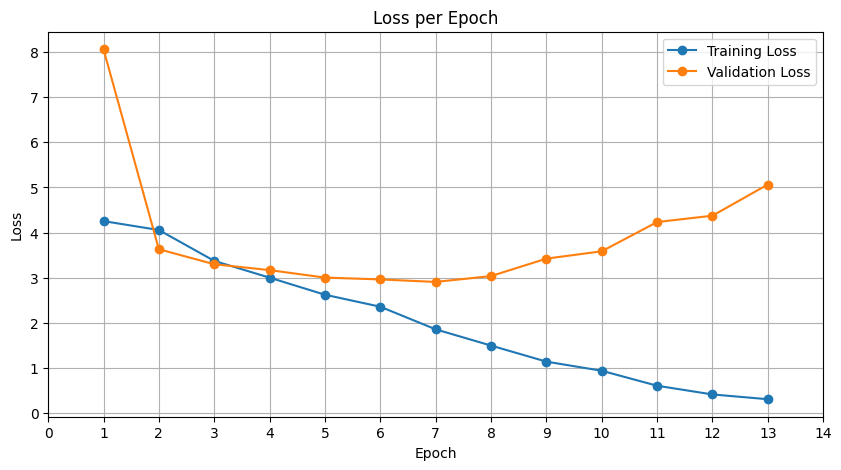
\includegraphics[width=\linewidth]{net6_loss.png}
        \caption{Net 6 CNN val vs training loss}
        \label{fig:net6_loss}
    \end{subfigure}
    \hfill
    \begin{subfigure}{0.45\linewidth}
        \centering
        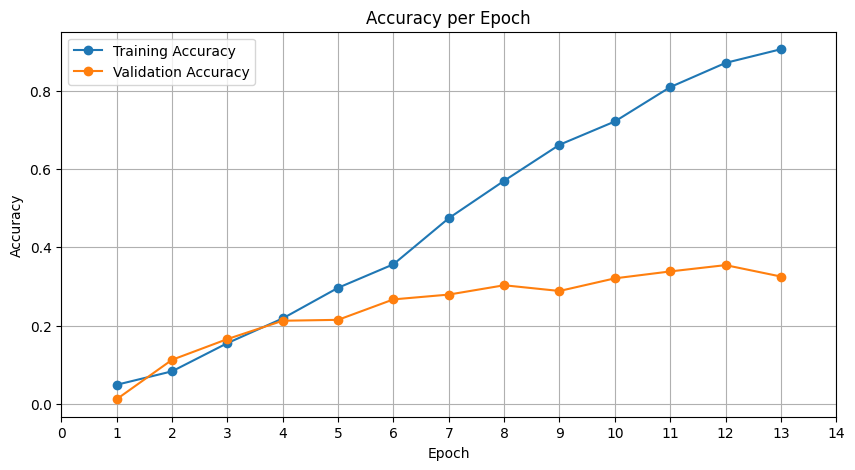
\includegraphics[width=\linewidth]{net6_acc.png}
        \caption{Net 6 CNN val vs training acc}
        \label{fig:net6_acc}
    \end{subfigure}
    \caption{Comparison of Net 6 performance}
    \label{fig:net6_performance}
\end{figure}

The model achieved a training accuracy of \textbf{90.6\%} at epoch 13, but the validation accuracy was significantly lower at \textbf{35.5\%}. This large gap between training and validation accuracy indicates \textbf{overfitting}, suggesting that the model fails to generalize to unseen data. Potential reasons for this performance include the relatively small dataset size and the high capacity of the model, which may require regularization techniques or data augmentation to improve generalization. Compared to its predecessor, NetCNN\_5, which achieved a training accuracy of \textbf{99.5\%} and a validation accuracy of \textbf{35.8\%}, NetCNN\_6 shows a lower training accuracy but a similar validation accuracy, indicating that while overfitting is still present, the model's training performance is more realistic. NetCNN\_6 introduces \textbf{five convolutional layers} with \textbf{stride-2} in some layers for downsampling and \textbf{average pooling} with kernel size 2 and stride 2 in multiple layers, aiming to improve feature extraction and model performance.

\section*{Comparison of all models}
Here's a summary of all models performance with highlighting on the key features each model has:

% \documentclass{article}
% \usepackage{amsmath}
% \usepackage{graphicx}
% \usepackage{array}

% \begin{document}
\begin{table}[ht]
    \centering
    \begin{tabular}{|c|c|c|p{6cm}|}
        \hline
        \textbf{Model} & \textbf{Training Accuracy} & \textbf{Validation Accuracy} & \textbf{Key Features} \\
        \hline
        NetCNN\_0 & 85.1\% & 30.3\% & Baseline model (3 layers) \\
        \hline
        NetCNN\_1 & 99.4\% & 24.3\% & Reduced to two convolutional layers \\
        \hline
        NetCNN\_2 & 99.1\% & 20.1\% & Batch normalization, dropout layer \\
        \hline
        NetCNN\_3 & 59.4\% & 54\% & Global Average Pooling (GAP) \\
        \hline
        NetCNN\_4 & 59.9\% & 55\% & Stride-2 convolutional layers \\
        \hline
        NetCNN\_5 & 99.5\% & 35.8\% & Four convolutional layers, alternating MaxPool and AvgPool \\
        \hline
        NetCNN\_6 & 90.6\% & 35.5\% & Five convolutional layers, stride=2 in some layers, average pooling \\
        \hline
    \end{tabular}
    \caption{Comparison of Models with Training and Validation Accuracy and Key Features}
    \label{tab:model_comparison}
\end{table}

Models NetCNN\_3 and NetCNN\_4 achieved the best performance with validation accuracies of \textbf{54\%} and \textbf{55\%}, respectively. This can be attributed to the introduction of \textbf{GAP} in NetCNN\_3, which helped reduce the number of parameters and improved generalization by replacing the fully connected layers. NetCNN\_4 further enhanced performance by incorporating \textbf{stride-2 convolutional layers} for downsampling, which allowed for more efficient feature extraction and reduced overfitting. In contrast, NetCNN\_0 and NetCNN\_1, the earlier models, struggled with overfitting and limited generalization due to their simpler architectures and lack of advanced regularization techniques. NetCNN\_2, despite introducing batch normalization and dropout layers, still suffered from a significant gap between training and validation accuracy, indicating overfitting. NetCNN\_5, with its four convolutional layers and alternating pooling operations, showed high training accuracy but failed to generalize well, resulting in a large gap between training and validation accuracy. NetCNN\_6, despite having a deeper architecture  and additional downsampling, also struggled with overfitting and did not achieve the same level of generalization as NetCNN\_3 and NetCNN\_4. Overall, the balance between model complexity and effective regularization in NetCNN\_3 and NetCNN\_4 contributed to their superior performance.




\section*{Task 2 Best Customized Model with augmentation}
In this section, the best model from the previous task was trained on the same data but this time, its augmented, so we can better notice the importance and effectivenss of the augmentaion process. 

The process of augmentation starts with applying various transformations and saving the augmented images. It iterates through each class directory within the input directory. For each image in the class directory, the function reads the image and applies a series of augmentations, including random rotation (± 20 degrees), random scale (± 50\%), random translation, and random illumination adjustment. Each augmented image is saved with a unique filename indicating the type of augmentation applied. The use of a progress bar provides a visual indication of the processing progress, enhancing the user experience by showing the status of the augmentation process. The net\_4 model was trained on the augmented data, and here's the results:


\begin{figure}[ht]
    \centering
    \begin{subfigure}{0.45\linewidth}
        \centering
        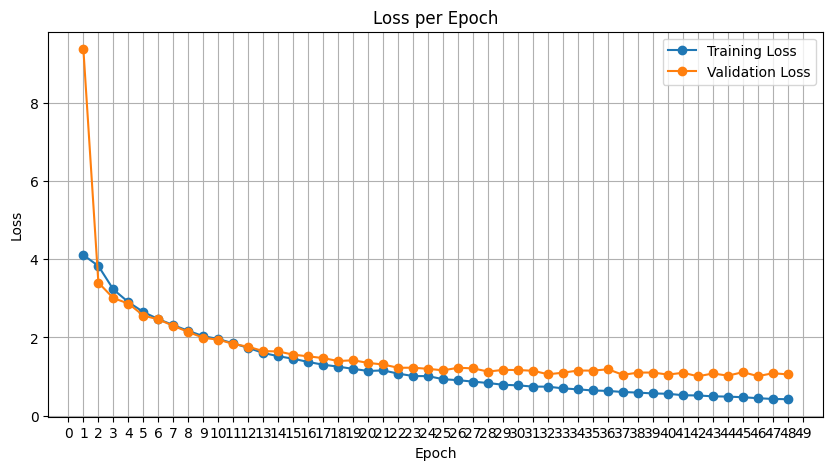
\includegraphics[width=\linewidth]{net4_aug_loss.png}
        \caption{Net 4 training vs validation loss with augmentation}
        \label{fig:net4_aug_loss}
    \end{subfigure}
    \hfill
    \begin{subfigure}{0.45\linewidth}
        \centering
        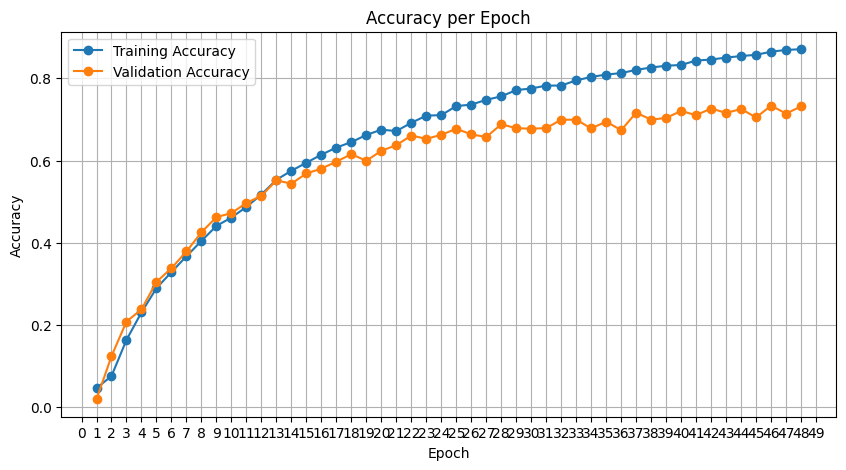
\includegraphics[width=\linewidth]{net4_aug_acc.png}
        \caption{Net 4 training vs validation acc with augmentation}
        \label{fig:net4_aug_acc}
    \end{subfigure}
    \caption{Net 4 performance with augmentation}
    \label{fig:net4_performance_with_augmentation}
\end{figure}


\begin{table}[ht]
    \centering
    \begin{tabular}{|c|c|c|}
        \hline
        \textbf{Metric} & \textbf{Without Augmentation} & \textbf{With Augmentation} \\
        \hline
        Training Loss & 0.309 & 0.421 \\
        \hline
        Validation Loss & 5.065 & 1.055 \\
        \hline
        Training Accuracy & 90.6\% & 87.1\% \\
        \hline
        Validation Accuracy & 35.5\% & 73.2\% \\
        \hline
    \end{tabular}
    \caption{Comparison of NetCNN\_4 Performance With and Without Augmentation}
    \label{tab:augmentation_comparison}
\end{table}

The table 2.2 compares the training loss, validation loss, training accuracy, and validation accuracy of NetCNN\_4 with and without augmentation. The effect of augmentation is highlighted by the significant improvement in validation accuracy (from 35.5\% to 73.2\%) and the reduction in validation loss (from 5.065 to 1.055), indicating augmentation helps the model generalize better to unseen data.



% \section*{Model Fine-Tuning and Training}

\section*{Task 3: Train Published CNN architecture}
In this section, Some well-known and published architectures were used to show their effect when trained on the AHAWP dataset, the models used are mobile net resnet-18 \& renset-50 and shallowe resnet architectures, all of models were adjusted to classify 82 classes by adding fully connected layer. Here's the results:

\textbf{Mobile net}


\begin{figure}[ht]
    \centering
    \begin{subfigure}{0.45\linewidth}
        \centering
        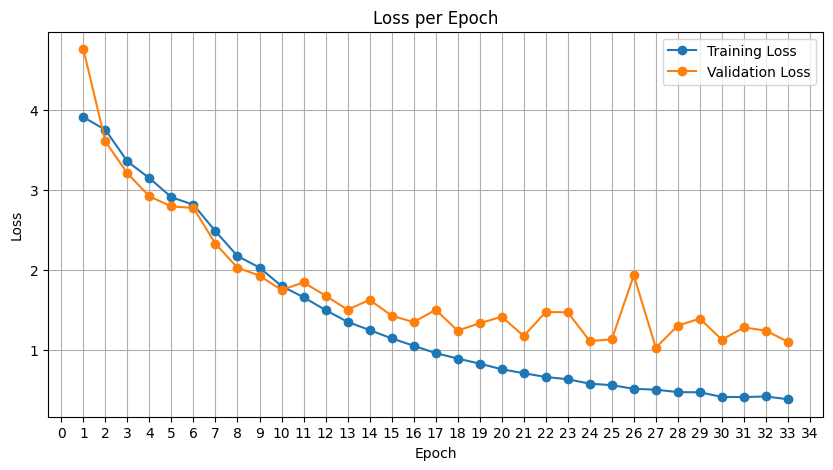
\includegraphics[width=\linewidth]{t3_mobilenet_loss.png}
        \caption{Mobilenet training vs val loss}
        \label{fig:t3_mobilenet_loss}
    \end{subfigure}
    \hfill
    \begin{subfigure}{0.45\linewidth}
        \centering
        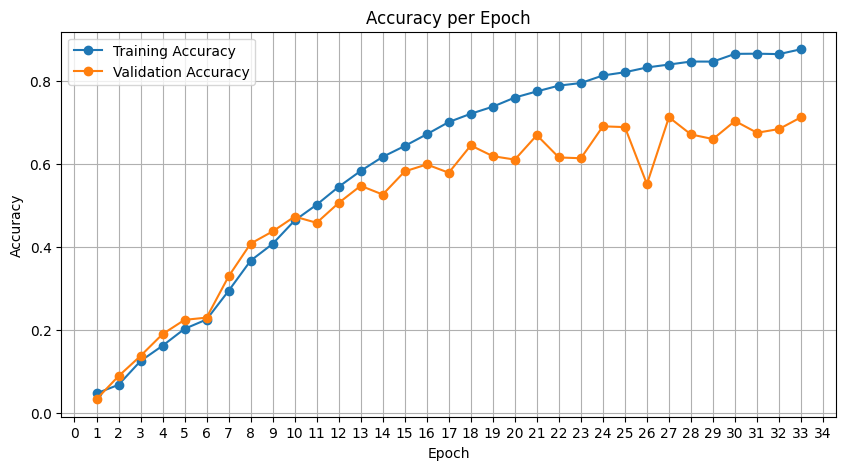
\includegraphics[width=\linewidth]{t3_mobilenet_acc.png}
        \caption{Mobilenet training vs val acc}
        \label{fig:t3_mobilenet_acc}
    \end{subfigure}
    \caption{Comparison of MobileNet performance}
    \label{fig:t3_mobilenet_performance}
\end{figure}

Mobilenet uses depthwise separable convolutions to reduce the number of parameters and computational cost while maintaining accuracy.

The model achieved a training accuracy of \textbf{87.6\%} at epoch 33, with a validation accuracy of \textbf{71.2\%}. The training loss was \textbf{0.384}, and the validation loss was \textbf{1.102}. This performance indicates that MobileNet is effective at generalizing to unseen data, balancing efficiency and accuracy.

\textbf{Resnet-18}


\begin{figure}[ht]
    \centering
    \begin{subfigure}{0.45\linewidth}
        \centering
        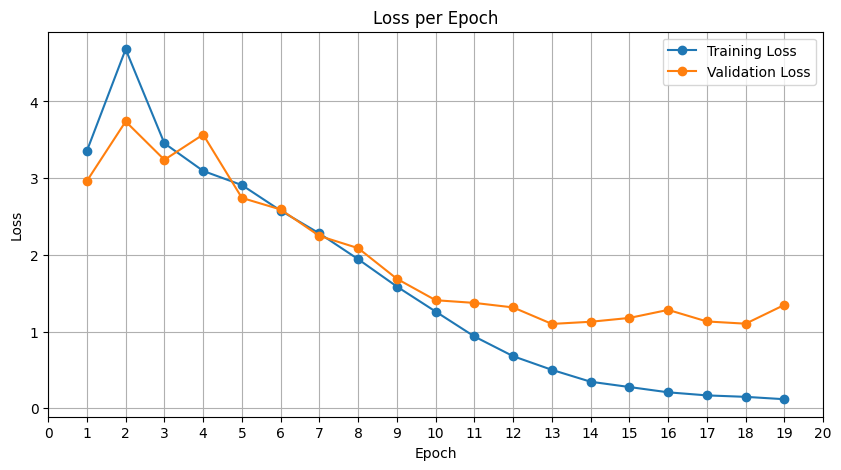
\includegraphics[width=\linewidth]{t3_res_18_loss.png}
        \caption{Resnet-18 training vs val loss}
        \label{fig:t3_res_18_loss}
    \end{subfigure}
    \hfill
    \begin{subfigure}{0.45\linewidth}
        \centering
        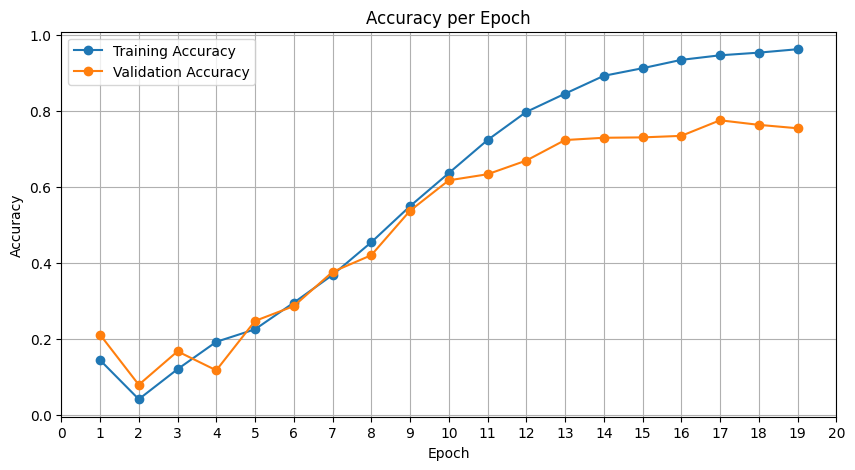
\includegraphics[width=\linewidth]{t3_res_18_acc.png}
        \caption{Resnet-18 training vs val acc}
        \label{fig:t3_res_18_acc}
    \end{subfigure}
    \caption{Comparison of ResNet-18 performance}
    \label{fig:t3_res_18_performance}
\end{figure}

ResNet-18  uses shortcut connections to skip one or more layers, allowing gradients to flow more easily during backpropagation.

The model achieved a training accuracy of \textbf{96.2\%} at epoch 19, with a validation accuracy of \textbf{77.5\%}. The training loss was \textbf{0.117}, and the validation loss was \textbf{1.347}. This performance indicates that ResNet-18 is highly effective at learning from the training data and generalizing to unseen data, although there is still some room for improvement in validation performance.



\textbf{Resnet-50}

\begin{figure}[ht]
    \centering
    \begin{subfigure}{0.45\linewidth}
        \centering
        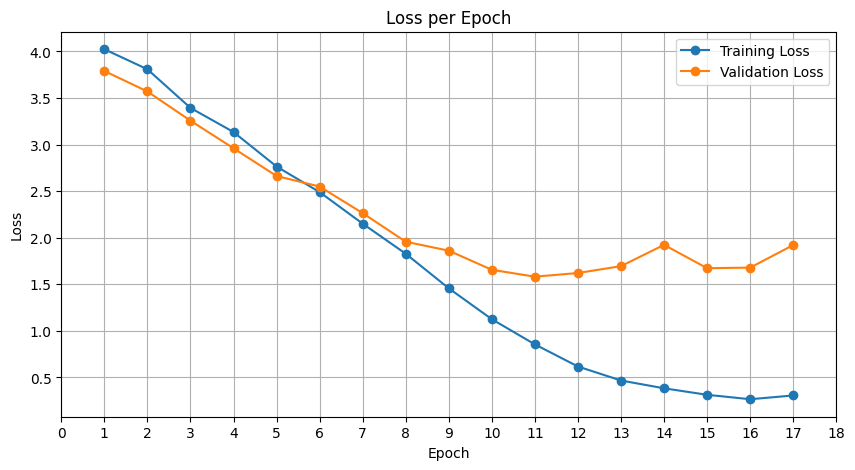
\includegraphics[width=\linewidth]{t3_res50_loss.png}
        \caption{Resnet-50 training vs val loss}
        \label{fig:t3_res50_loss}
    \end{subfigure}
    \hfill
    \begin{subfigure}{0.45\linewidth}
        \centering
        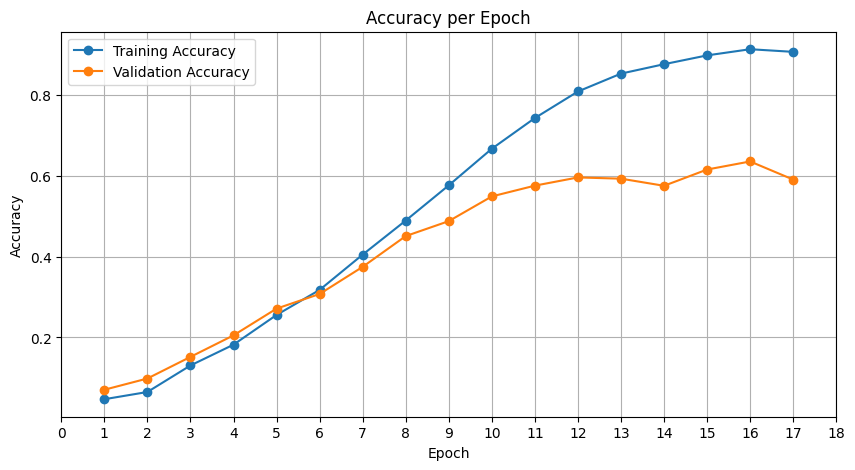
\includegraphics[width=\linewidth]{t3_res50_acc.png}
        \caption{Resnet-50 training vs val acc}
        \label{fig:t3_res50_acc}
    \end{subfigure}
    \caption{Comparison of ResNet-50 performance}
    \label{fig:t3_res50_performance}
\end{figure}

ResNet-50 extends the ResNet family by using 50 layers with residual connections, allowing for improved gradient flow and deeper network training. It employs bottleneck layers to reduce the number of parameters while maintaining performance.

The model achieved a training accuracy of \textbf{90.7\%} at epoch 17, with a validation accuracy of \textbf{63.6\%}. The training loss was \textbf{0.307}, and the validation loss was \textbf{1.922}. This performance indicates that ResNet-50 is effective at learning from the training data, but there is a noticeable gap between training and validation accuracy, suggesting potential overfitting and room for improvement in generalization.



\textbf{Shallow Resnet}



\begin{figure}[ht]
    \centering
    \begin{subfigure}{0.45\linewidth}
        \centering
        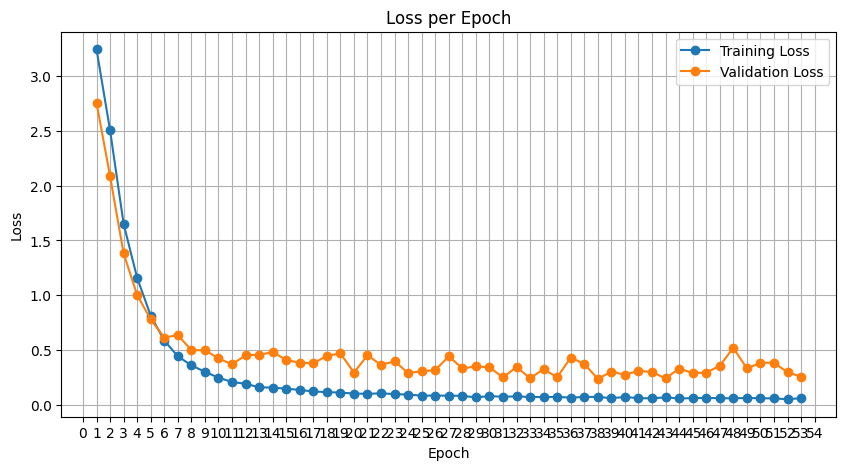
\includegraphics[width=\linewidth]{t3_sh_res_loss.png}
        \caption{Shallow Resnet training vs val loss}
        \label{fig:t3_sh_res_loss}
    \end{subfigure}
    \hfill
    \begin{subfigure}{0.45\linewidth}
        \centering
        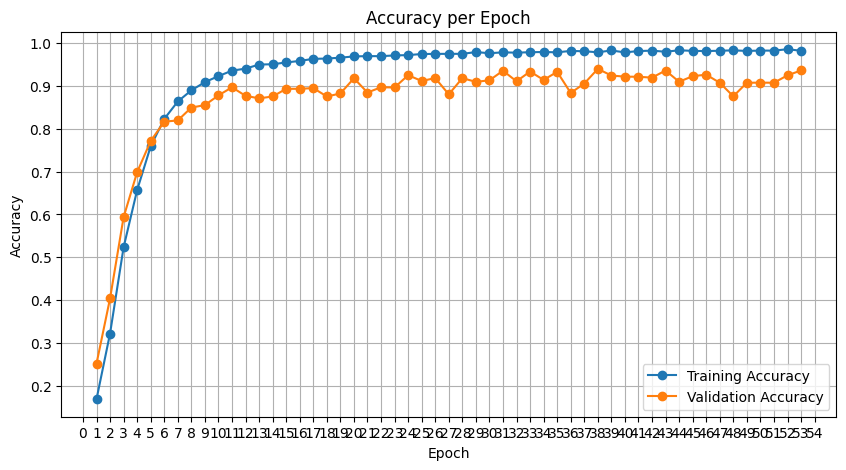
\includegraphics[width=\linewidth]{t3_sh_res_acc.png}
        \caption{Shallow Resnet training vs val acc}
        \label{fig:t3_sh_res_acc}
    \end{subfigure}
    \caption{Comparison of Shallow ResNet performance}
    \label{fig:t3_sh_res_performance}
\end{figure}

The customized Shallow ResNet is a convolutional neural network that uses residual blocks to improve gradient flow and ease the training of deep networks. It consists of multiple convolutional layers with batch normalization, ReLU activation, and adaptive average pooling, followed by a fully connected layer \href{https://github.com/XavierSpycy/EMNIST-Classifier/tree/main?tab=readme-ov-file&fbclid=IwZXh0bgNhZW0CMTEAAR28TUMKmsi-__lqn5Kghur0N787OLz2i_F1VS9roCK0PDzmlKxDdLlqj3A_aem_w7o4e13T9U_QePSc0L5I3Q#sparkles-6-pre-training--fine-tuning}{Shallow Resnet Classifier on GitHub}.

The model achieved a training accuracy of \textbf{98.2\%} at epoch 53, with a validation accuracy of \textbf{94.0\%}. The training loss was \textbf{0.059}, and the validation loss was \textbf{0.257}. This performance indicates that the Shallow ResNet is highly effective at learning from the training data and generalizing to unseen data, demonstrating strong overall performance.

\section*{Comparison Published architectures Models}


\begin{table}[ht]
    \centering
    \begin{tabular}{|c|c|c|p{6cm}|}
        \hline
        \textbf{Model} & \textbf{Training Accuracy} & \textbf{Validation Accuracy} & \textbf{Key Features} \\
        \hline
        NetCNN\_4 & 59.9\% & 55\% & Stride-2 convolutional layers \\
        \hline
        MobileNet & 87.6\% & 71.2\% & Depthwise separable convolutions \\
        \hline
        ResNet-18 & 96.2\% & 77.5\% & Residual connections, 18 layers \\
        \hline
        ResNet-50 & 90.7\% & 63.6\% & Residual connections, 50 layers \\
        \hline
        Shallow ResNet & 98.2\% & 94.0\% & Customized shallow architecture with residual blocks \\
        \hline
    \end{tabular}
    \caption{Comparison of Model Performance}
    \label{tab:model_comparison}
\end{table}

The Shallow ResNet achieved the best performance with a training accuracy of \textbf{98.2\%} and a validation accuracy of \textbf{94.0\%}. This superior performance can be attributed to its customized shallow architecture with residual blocks, which effectively improves gradient flow and eases the training of deep networks. The use of residual connections helps prevent the vanishing gradient problem, allowing the model to learn more complex features and generalize better to unseen data. Additionally, the combination of batch normalization and ReLU activation further enhances the model's training stability and performance.

In contrast, ResNet-18 and ResNet-50, despite their deeper architectures, failed to achieve the same level of performance. ResNet-18 achieved a training accuracy of \textbf{96.2\%} and a validation accuracy of \textbf{77.5\%}, while ResNet-50 achieved a training accuracy of \textbf{90.7\%} and a validation accuracy of \textbf{63.6\%}. One reason for this discrepancy is that the deeper networks are more prone to overfitting, especially when trained on smaller datasets. Additionally, the Shallow ResNet was trained with a patience of 10, allowing it more epochs to improve and stabilize, whereas ResNet-18 and ResNet-50 were trained with a patience of 6, potentially leading to earlier stopping and less optimal performance.


\section*{Task 4 : Fine Tune Published Pretrained Models}
The same Model were used as in Task3, but with their pretraiend weights on the Imagenet dataset, and here are the results:

\textbf{Mobilenet}

\begin{figure}[ht]
    \centering
    \begin{subfigure}{0.45\linewidth}
        \centering
        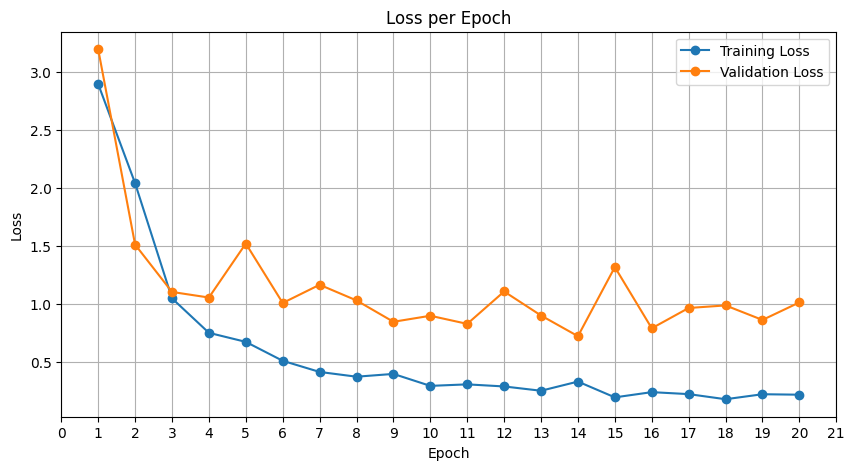
\includegraphics[width=\linewidth]{t4_mobilenet_loss.png}
        \caption{Pretrained Mobilenet training vs val loss}
        \label{fig:t4_mobilenet_loss}
    \end{subfigure}
    \hfill
    \begin{subfigure}{0.45\linewidth}
        \centering
        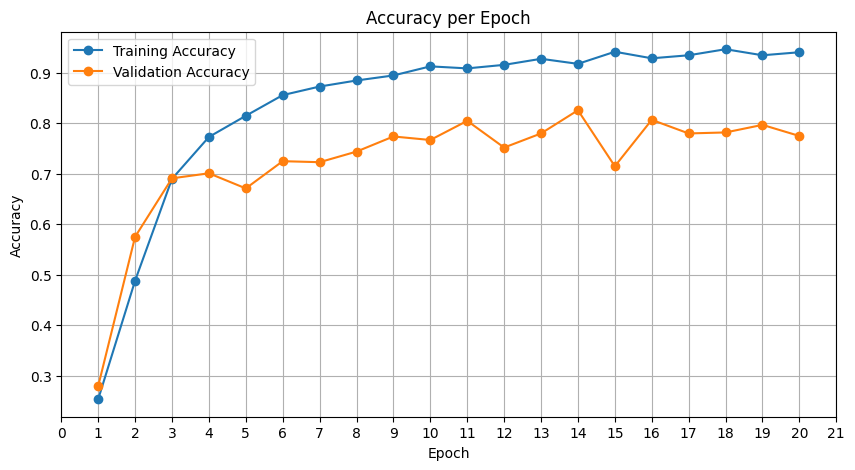
\includegraphics[width=\linewidth]{t4_mobilenet_acc.png}
        \caption{Pretrained Mobilenet training vs val acc}
        \label{fig:t4_mobilenet_acc}
    \end{subfigure}
    \caption{pretrained MobileNet performance}
    \label{fig:t4_mobilenet_performance}
\end{figure}

The pretrained MobileNet model achieved a training accuracy of \textbf{92.9\%} and a validation accuracy of \textbf{80.7\%} at epoch 20. The training loss was \textbf{0.238}, and the validation loss was \textbf{0.788}. Early stopping was applied due to the validation loss increasing for 6 consecutive epochs at epoch 20. This performance indicates that MobileNet is highly effective at learning from the training data and generalizing to unseen data. The relatively high validation accuracy and low validation loss demonstrate that the model maintains a good balance between efficiency and accuracy, making it suitable for mobile and embedded vision applications. The use of depthwise separable convolutions in MobileNet helps reduce the number of parameters and computational cost while maintaining strong performance, contributing to its effectiveness in real-world scenarios.


\textbf{Resnet-50}


\begin{figure}[ht]
    \centering
    \begin{subfigure}{0.45\linewidth}
        \centering
        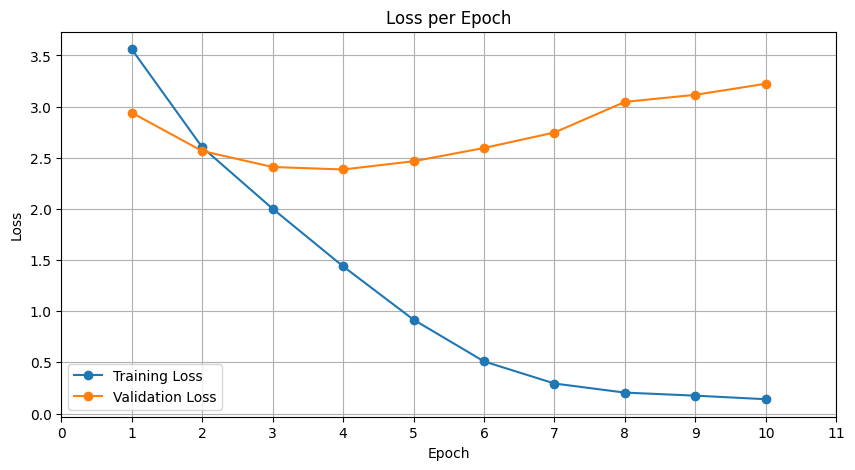
\includegraphics[width=\linewidth]{t4_res50_loss.png}
        \caption{ResNet-50 training vs validation loss}
        \label{fig:t4_res50_loss}
    \end{subfigure}
    \hfill
    \begin{subfigure}{0.45\linewidth}
        \centering
        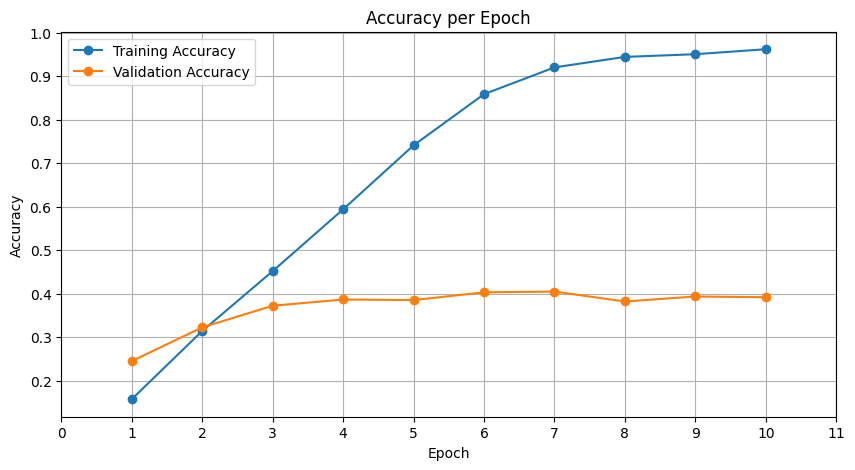
\includegraphics[width=\linewidth]{t4_res50_acc.png}
        \caption{ResNet-50 training vs validation accuracy}
        \label{fig:t4_res50_acc}
    \end{subfigure}
    \caption{Comparison of ResNet-50 performance}
    \label{fig:t4_res50_performance}
\end{figure}

The pretrained ResNet-50 model achieved a training accuracy of \textbf{92.1\%} and a validation accuracy of \textbf{40.5\%} at epoch 7. The training loss was \textbf{0.293}, and the validation loss was \textbf{2.746}. Early stopping was applied due to the validation loss. This performance indicates that while ResNet-50 is highly effective at learning from the training data, it struggles to generalize to unseen data, as evidenced by the significant gap between training and validation accuracy. The high validation loss further suggests that the model is overfitting to the training data. Despite its deeper architecture and the use of residual connections to improve gradient flow, ResNet-50's performance in this scenario highlights the challenges of training deep networks on smaller datasets without sufficient regularization or data augmentation techniques.


\subsection*{Comparison Between Pretrained and untrained models}

\begin{table}[ht]
    \centering
    \begin{tabular}{|c|c|c|}
        \hline
        \textbf{Model} & \textbf{Training Accuracy} & \textbf{Validation Accuracy} \\
        \hline
        Unpretrained ResNet-50 & 90.7\% & 63.6\% \\
        \hline
        Pretrained ResNet-50 & 92.1\% & 40.5\% \\
        \hline
        Unpretrained MobileNet & 87.6\% & 71.2\% \\
        \hline
        Pretrained MobileNet & 92.9\% & 80.7\% \\
        \hline
    \end{tabular}
    \caption{Comparison of Model Performance}
    \label{tab:model_comparison}
\end{table}

\textbf{Evaluation:} The unpretrained ResNet-50 model achieved a training accuracy of \textbf{90.7\%} and a validation accuracy of \textbf{63.6\%}, indicating a reasonable balance between training and validation performance. In contrast, the pretrained ResNet-50 model achieved a slightly higher training accuracy of \textbf{92.1\%} but a significantly lower validation accuracy of \textbf{40.5\%}. The pretrained model's higher training accuracy suggests that it was able to learn the training data more effectively, but the lower validation accuracy indicates that it struggled to generalize to unseen data. This discrepancy may be due to the pretrained weights being optimized for a different dataset, leading to overfitting when fine-tuned on the current dataset. 

The unpretrained MobileNet model achieved a training accuracy of \textbf{87.6\%} and a validation accuracy of \textbf{71.2\%}, demonstrating good generalization. The pretrained MobileNet model, with a training accuracy of \textbf{92.9\%} and a validation accuracy of \textbf{80.7\%}, showed the best generalization among the models. The use of depthwise separable convolutions in MobileNet helps reduce the number of parameters and computational cost while maintaining strong performance, contributing to its effectiveness in real-world scenarios. The pretrained weights further enhance its performance by providing a strong initialization based on a large dataset.


\clearpage

\section*{Conclusion}

In this project, we utilized the AHAWP dataset to train and evaluate various convolutional neural network (CNN) architectures. The dataset underwent preprocessing and augmentation to enhance the model's ability to generalize to unseen data. Preprocessing steps included resizing images to a consistent input size of \(1 \times 224 \times 224\) and normalizing pixel values. Augmentation techniques such as random rotation, translation, illumination adjustment, and scaling were applied to increase the diversity of the training data and reduce overfitting.

We evaluated several models, including NetCNN\_4, MobileNet, ResNet-18, ResNet-50, and a customized Shallow ResNet. Each model was assessed based on its training and validation accuracy, as well as its ability to generalize to unseen data. The results of these evaluations are summarized in the following table:

\begin{table}[ht]
    \centering
    \begin{tabular}{|c|c|c|}
        \hline
        \textbf{Model} & \textbf{Training Accuracy} & \textbf{Validation Accuracy} \\
        \hline
        NetCNN\_4 & 59.9\% & 55\% \\
        \hline
        Unpretrained ResNet-50 & 90.7\% & 63.6\% \\
        \hline
        Pretrained ResNet-50 & 92.1\% & 40.5\% \\
        \hline
        Unpretrained MobileNet & 87.6\% & 71.2\% \\
        \hline
        Pretrained MobileNet & 92.9\% & 80.7\% \\
        \hline
        Shallow ResNet & 98.2\% & 94.0\% \\
        \hline
    \end{tabular}
    \caption{Comparison of Model Performance}
    \label{tab:model_comparison}
\end{table}

In Task 1, we evaluated basic CNN architectures like NetCNN\_4, which achieved a validation accuracy of 55\%. Task 2 focused on MobileNet, with the pretrained version reaching 80.7\% validation accuracy, highlighting the benefits of transfer learning. Task 3 involved ResNet-18 and ResNet-50 models, where the unpretrained ResNet-50 achieved 63.6\% validation accuracy, while the pretrained version struggled with 40.5\% due to overfitting.

The best-performing model was the customized Shallow ResNet, with a training accuracy of 98.2\% and a validation accuracy of 94.0\%. Its superior performance is due to its shallow architecture with residual blocks, which improve gradient flow and prevent the vanishing gradient problem. Batch normalization and ReLU activation further enhance training stability. Additionally, training with a patience of 10 allowed more epochs for improvement and stabilization.


\section*{Future Work}

While the project achieved promising results, several areas for improvement have been identified. Overfitting was a significant challenge, particularly with the pretrained ResNet-50 model. Future work could focus on implementing robust regularization techniques such as dropout, weight decay, increasing the dataset size, and advanced data augmentation strategies. Additionally, addressing the issue of loss fluctuation by adjusting learning rates and using more stable optimization algorithms could help stabilize the training process. Exploring different architectures like EfficientNet or DenseNet, hyperparameter optimization, and advanced training techniques, such as learning rate scheduling and ensemble methods, could further enhance performance. Incorporating comprehensive evaluation metrics, such as precision, recall, and F1-score, would provide a more detailed assessment of the model's performance. These efforts could lead to better performance and more robust models for real-world applications.


\end{document}


\end{document}
